\section{22.02.24 : Wstęp - homotopijna równoważność, pojęcie grupy podstawowej}

\subsection{Drogi, homotopijna równoważność}

W przestrzeni topologicznej $X$ \buff{droga} między punktami $x_0$ a $x_1$ to ciągła funkcja $f:[0,1]\to X$ taka, że $f(0)=x_0$ oraz $f(1)=x_1$.

\begin{definition}[homotopia]
  Niech $f_t$ dla $t\in[0,1]$ będzie rodziną dróg między $x_0$ a $x_1$ w $X$ takich, że
  \begin{itemize}
    \item dla każdego $t\in[0,1]$ $f_t(0)=x_0$ oraz $f_t(1)=x_1$;
    \item rodzina ta zależy w sposób ciągły od $t$, tzn. istnieje przekształcenie ciągłe $F:[0,1]\times[0,1]\to X$ takie, że $F(s, t)=f_t(s)$.
  \end{itemize}
  Przekształcenie $F$ nazywamy \buff{homotopią} między $f_0$ a $f_1$.
\end{definition}

Możemy to zobrazować albo jako ciągłe przeciąganie dwóch sznurków:
\begin{center}
  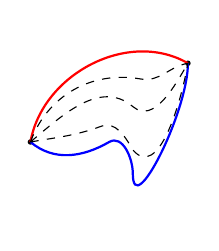
\begin{tikzpicture}
    \fill (2, 1) circle (1pt);
    \fill (0,0) circle (1pt);

    \draw[red, thick] (0,0) to[out=80, in=150] (2, 1);
    \draw[blue, thick] (0,0) to[out=-40, in=210] (1, 0) to[out=30, in=90] (1.3, -0.4) to[out=-90, in=-90] (2, 1);

    \draw[dashed] (0,0) to[out=40, in=140] (1.3, 0.45) to[out=-40, in=-120] (2, 1);
    \draw[dashed] (0,0) to[out=70, in=170] (1.4, 0.8) to[out=-10, in=190] (2, 1);
    \draw[dashed] (0,0) to[out=10, in=200] (0.9, 0.2) to[out=20, in=120] (1.3, -0.1) to[out=-50, in=-100] (2, 1);
  \end{tikzpicture}
\end{center}
lub, bardziej abstrakcyjnie, jako kwadrat, który $F$ przeprowadza w $X$:
\begin{center}
  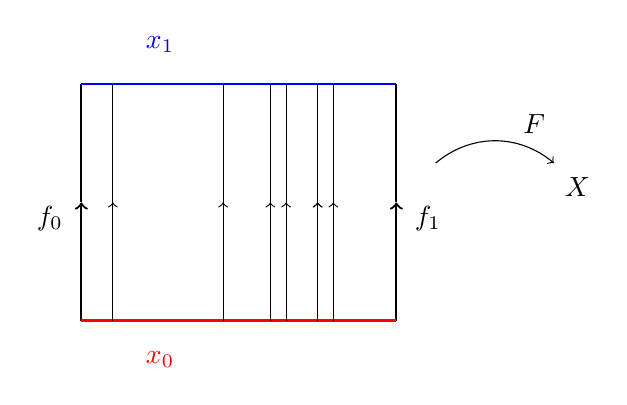
\begin{tikzpicture}
    \draw[->, thick](0,0)--(0, 1.5);
    \draw[thick] (0, 1.5)--(0, 3);
    \draw[blue, thick] (0, 3)--(4, 3);
    \draw[->, thick] (4, 0)--(4, 1.5);
    \draw[thick](4, 1.5)--(4, 3);
    \draw[red, thick](0,0)--(4, 0);

    \foreach \i in {0, 1, ..., 6} {
      \coordinate (z\i) at ({random(2, 18) * 1/5}, 0);
      \draw[->] (z\i) -- ++(0, 1.5);
      \draw (z\i) -- ++(0, 3);
    } 
    
    \node at (-0.4, 1.3) {$f_0$};
    \node at (4.4, 1.3) {$f_1$};

    \node at (1, 3.5) {$\color{blue} x_1$};
    \node at (1, -.5) {$\color{red} x_0$};

    \draw[->] (4.5, 2) to [out=40, in=140] (6, 2);
    \node at ({4.5 + 1.25}, 2.5) {$F$};
    \node at (6.3, 1.7) {$X$};
  \end{tikzpicture}
\end{center}

Jeśli za $X$ weźmiemy $\R^n$, to każde dwie drogi $f, g:[0,1]\to \R^n$ o wspólnym początku są homotopijne. Możemy np. napisać tzw. homotopię "liniową":
$$F(x, t)=(1-t)f(s)+t\cdot g(s).$$
To samo tyczy się dowolnego wypukłego podzbioru $A\subseteq\R^n$.

\begin{fact}
  Homotopijność dróg jest jest relacją równoważności na zbiorze wszystkich dróg od $x_0$ do $x_1$ w $X$.
\end{fact}

Jest więc sensownym rozważanie klas abstrakcji relacji homotopijnej równoważności dróg. Przez $\color{blue}\boldsymbol{[f]}$ będziemy zwykle rozumieć klasę dróg homotopijnych z $f$.

\begin{proof}
  Niech $f, g, h:[0,1]\to X$ będą drogami między $x_0$ a $x_1$ takimi, że $f$ jest homotopijna z $g$, a $g$ jest homotopijna z $h$.

  \begin{enumerate}
    \item Zwrotność: oczywista homotopia między $f$ a $f$ to identyczność: $F(t, s)=f(t)$.
    \item Symetryczność: niech $F$ będzie homotopią między $f$ i $g$ (tzn. $F(t, 0)=f(t)$, $F(t, 1)=g(t)$). Wtedy $G(t, s)=F(t, 1-s)$ spełnia $G(t, 0)=F(t, 1)=g(t)$ oraz $G(t, 1)=F(t, 0)=f(t)$, czyli $G$ jest homotopią między $g$ a $f$. Ciągłość tego odwzorowania wynika z ciągłości $F$ oraz odwzorowania $x\mapsto 1-x$.
    \item Przechodność: niech $F$ będzie homotopią miedzy $f$ i $g$, a $G$ - między $g$ a $h$. Wtedy 
      $$H(t, s)=
      \begin{cases}
        F(t, 2\cdot s) & s\leq \frac{1}{2}\\ 
        G(t, 2s-1) & s>\frac{1}{2}.
      \end{cases}$$
      Widać, że $H(t, 0)=F(t, 2\cdot 0)=f(t)$ oraz $H(t, 1)=G(t, 2-1)=h(t)$. Ciągłość może psuć się wyłącznie w $s=\frac{1}{2}$ i wystarczy zauważyć, że granica idąc od lewej i idąc od prawej wynosi $g(t)$.
  \end{enumerate}
\end{proof}

Składając drogi chcemy, aby wynik tego działania nadal był drogą. W takim razie, musimy pilnować, aby koniec pierwszej drogi i początek drugiej były tym samym punktem, oraz aby złożenie było funkcją z $[0,1]$.

\begin{definition}[złożenie dróg]
  Niech $f,g:[0,1]\to X$ będą drogami takimi, że $f(1)=g(0)$. Wtedy 
  $$fg(s):=\begin{cases}f(2s)&s\leq\frac{1}{2}\\ g(2s-1) & s>\frac{1}{2}\end{cases}$$
  jest złożeniem dróg $f$ i $g$. Piszemy czasem $fg=f\cdot g$.
\end{definition}

\begin{fact}\label{fakt:1.2}
  Jeśli $f\sim f'$ oraz $g\sim g'$ są parami homotopijnych dróg, $f(1)=g(0)$ oraz $f'(1)=g'(0)$, to $fg\sim f'g'$.
\end{fact}

Z tego wynika, że możemy mówić o \acc{składaniu klas homotopii}, tzn.: 
$$\color{blue}\boldsymbol{[f][g]=[fg]}.$$

\begin{lemma}[łączność]\label{lemma:1.3}
  Działanie składania klas homotopii, o ile ma sens, jest działaniem łącznym. To znaczy, że 
  $$[(fg)h]=([f][g])[h]=[f]([g][h])=[f(gh)].$$
\end{lemma}

\begin{proof}
  Wystarczy pokazać, że $(fg)h\sim f(gh)$. Rysunkowo, wygląda to tak:
  \begin{center}
    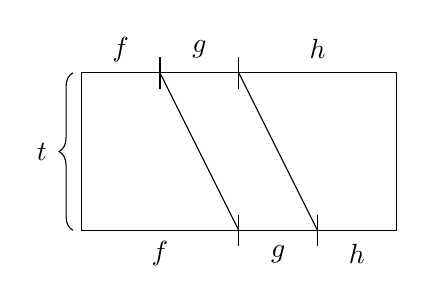
\begin{tikzpicture}
      \draw (0,0) rectangle ++(4, 2);
      \draw (2, 1.8)--(2, 2.2);
      \draw (1, 1.8)--(1, 2.2);

      \draw (2, 0.2)--(2, -0.2);
      \draw (3, 0.2)--(3, -0.2);
      
      \draw (2, 0)--(1, 2);
      \draw (3, 0)--(2, 2);

      \node at (0.5, 2.3) {$f$};
      \node at (1.5, 2.3) {$g$};
      \node at (3, 2.3) {$h$};
    
      \node at (1, -.3) {$f$};
      \node at (2.5, -.3) {$g$};
      \node at (3.5, -.3) {$h$};

      \draw[decorate, decoration={brace, amplitude=5pt, mirror, raise=4ex}] (0.5, 2) -- (0.5, 0);
      \node at (-0.5, 1) {$t$};
    \end{tikzpicture}
  \end{center}
  natomiast homotopia jawnie wyraża się
  $$F(s, t)=\begin{cases}
    f((4-2t)s)&s\leq \frac{1}{2(2-t)}\\ 
    g(4s-(1+t))&\frac{1+t}{4}<s\leq \frac{2+t}{4}\\ 
    h((2+2t)s-(1+2t))&\frac{1+2t}{2+2t}<s
  \end{cases}$$
\end{proof}

\subsection{Grupa podstawowa}

\begin{definition}[pętla]
  Pętla w $X$ zbazowana w punkcie $x_0\in X$ to droga w $X$ o początku i końcu $x_0$.
\end{definition}

Złożenie pętli zawsze ma sens i zawsze daje pętle zbazowaną w $x_0$.

\begin{theorem}[$\Pi_1(X, x_0)$]\label{twierdzenie:1.4}
  Zbiór wszystkich klas abstrakcji pętli zbazowanych w $x_0$, oznaczany $\color{blue}\boldsymbol{\Pi_1(X, x_0)}$, z działaniem składania dróg jest grupą. 
\end{theorem}

Zbiór $\Pi_1(X, x_0)$ nazywamy \buff{grupą podstawową} $X$ z wyróżnionym punktem $x_0$.

\begin{proof}
  Łączność tego działania jest jasna z \ref{lemma:1.3}. Elementem neutralnym jest pętla stale równa $x_0$, którą oznaczamy $x_0:[0,1]\to X$, $x_0(s)=x_0$. Aby zauważyć, że dla dowolnej pętli $f$ zachodzi $f=fx_0=x_0f$, wystarczy zauważyć, że $fx_0$ oraz $x_0f$ jest po prostu zmianą parametryzacji $f$:
  \begin{center}
    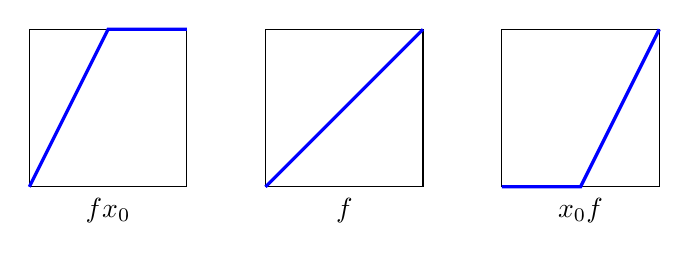
\begin{tikzpicture}
      \draw (0,0) rectangle ++ (2, 2);
      \draw[very thick, blue] (0,0)--(2,2);

      \draw(3, 0) rectangle ++(2, 2);
      \draw[very thick, blue](3, 0)--(4, 0)--(5, 2);

      \draw (-3, 0) rectangle ++(2,2);
      \draw[very thick, blue](-3, 0)--(-2, 2)--(-1, 2);

      \node at (1, -0.3) {$f$};
      \node at (4, -0.3) {$x_0f$};
      \node at (-2, -0.3) {$fx_0$};
    \end{tikzpicture}
  \end{center}
  czyli podobnie jak w dowodzie \ref{lemma:1.3} możemy napisać homotopię między tymi drogami.

  Pozostaje sprawdzić, czy dowolna droga $f$ posiada element odwrotny. Rozważmy $f'(t)=f(1-t)$, czyli $f$ przechodzone "od tyłu". Rozważmy homotopię 
  $$F(s, t)=\begin{cases}
    f(2s) & s\leq \frac{1-t}{2}\\ 
    f(1-t) & \frac{1-t}{2}<s\leq \frac{t+1}{2}\\ 
    f(2-2s) & \frac{1+t}{2}\leq s
  \end{cases}$$
  która dla $t=0$ jest równa $F(s, 0)=ff'(s)$, a dla $t=1$ staje się funkcją stałą $F(s, 1)=x_0$. Graficznie, można to przedstawić jako
  \begin{center}
    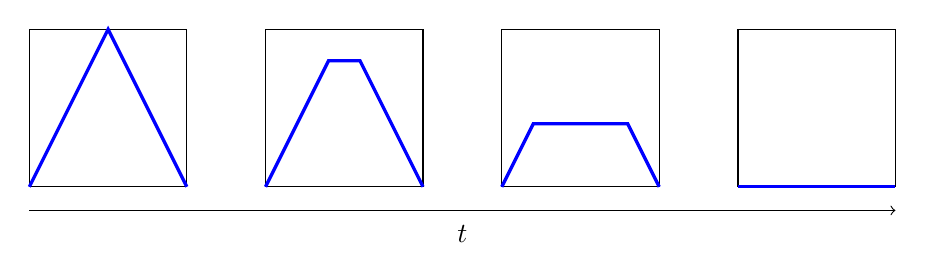
\begin{tikzpicture}
      \draw (0,0) rectangle ++(2,2);
      \draw[very thick, blue] (0,0)--(1, 2)--(2,0);

      \draw (3, 0) rectangle ++(2,2);
      \draw[very thick, blue] (3, 0)--(3.8, 1.6)--(4.2, 1.6)--(5, 0);

      \draw (6, 0) rectangle ++(2,2);
      \draw[very thick, blue] (6, 0)--(6.4, 0.8)--(7.6, 0.8)--(8, 0);

      \draw (9, 0) rectangle ++(2, 2);
      \draw[very thick, blue] (9, 0)--(11, 0);

      \draw[->] (0, -0.3)--(11, -0.3);
      \node at (5.5, -0.6) {$t$};

      %\draw[->] (-.3, 0)--(-.3, 2);
      %\node at (-.6, 1) {$s$};
    \end{tikzpicture}
  \end{center}
\end{proof}

\begin{example}
  \item Dla dowolnego wypukłego podzbioru $A\subseteq\R^n$ i dowolnego punktu $x_0\in A$ grupa podstawowa $\Pi_1(A, x_0)=0$ jest trywialna, gdyż każde dwie drogi są homotopijnie równoważne.
  \item Jeśli $X=S^1$, to bez względu na wybór $x_0\in X$ mamy $\Pi_1(X, x_0)=\Z$. Można to sobie wyobrazić jako zakręcanie $n$ pętli nad $S^1$:
    \begin{center}
      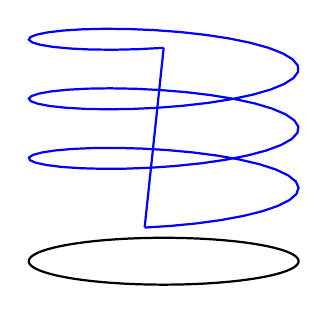
\begin{tikzpicture}
        \begin{axis} [
          view={0}{30},
          axis lines=none,
          ymin=-2,
          ymax=5,
          xmin=-2,
          xmax=2]
      
          \addplot3 [thick, blue, domain=3:7*pi, samples = 100, samples y=0] ({sin(deg(-x))}, {cos(deg(-x))}, {x});
          \addplot3 [thick, domain=0:2*pi, samples = 100, samples y=0] ({sin(deg(x))}, {cos(deg(x))}, -3);
          %\addplot3 [thick, only marks, blue, mark=o] ({sin(deg(-3))}, {cos(deg(-3)}, {3});

          \addplot3[thick, blue] coordinates{ ({sin(deg(-3))}, {cos(deg(-3))}, 3) ({sin(deg(-7*pi))}, {cos(deg(-7*pi))}, 7*pi )};
      \end{axis}
      \end{tikzpicture}
    \end{center}
\end{example}

Naturalne będzie teraz pytanie, jak bardzo $\Pi_1(X, x_0)$ zależy od wyboru punktu $x_0$? 

\begin{lemma}\label{lemma:1.5}
  Niech $h:[0,1]\to X$ będzie drogą od $x_0$ do $x_1$. Wówczas istnieje odwzorowanie 
  $$\beta_h:\Pi_1(X, x_0)\to \Pi_1(X, x_1)$$
  zadane przez 
  $$\beta_h([f])=[hfh^{-1}],$$
  które jest izomorfizmem grup.
\end{lemma}

\begin{proof}
  Po pierwsze, jeśli $F$ jest homotopią dróg $f$ i $g$ w $\Pi_1(X, x_0)$, to $G(t, _)=hF(t,-)h^{-1}$ jest homotopią $hfh^{-1}$ oraz $hgh^{-1}$, czyli pętli zbazowanych w $x_1$. W takim razie, odwzorowanie jest dobrze zdefiniowane (klasy abstrakcji przechodzą na klasy abstrakcji).

  $\beta_h$ jest też homomorfizmem grup, bo 
  $$\beta_h[fg]=[h(fg)h^{-1}]=[(hfh^{-1})(hgh^{-1})]=[hfh^{-1}][hgh^{-1}]=\beta_h[f]\beta_h[g].$$
  
  Dodatkowo, $\beta_{h^{-1}}[f]=[h^{-1}fh]$ jest odwrotnością $\beta_h$:
  $$\beta_h\beta_{h^{-1}}[f]=\beta_h[h^{-1}fh]=[h(h^{-1}fh)h^{-1}]=[f]$$
  oraz podobnie $\beta_{h^{-1}}\beta_h[f]=[f]$.
\end{proof}

Przypomnijmy, że przestrzeń $X$ jest łukowo spójna, jeśli dla dowolnych dwóch punktów $x, y\in X$ istnieje droga między nimi.

\begin{uwaga}
  Na mocy \ref{lemma:1.5} wszystkie grupy podstawowe łukowo spójnej przestrzeni $X$ są parami izomorficzne. Możemy więc opuścić pamiętanie punktu bazowego i pisać po prostu $\Pi_1(X)$.
\end{uwaga}

\subsection{Homomorfizmy indukowane}

Niech $X$ będzie przestrzenią topologiczną z wyróżnionym punktem $x_0$, a $Y$ - przestrzenią z wyróżnionym punktem $y_0$. Odwzorowanie ciągłe $\phi:X\to Y$, które zachowuje punkt wyróżniony (tzn. $\phi(x_0)=y_0$) zapisujemy czasem jako odwzorowanie 
$$\phi:(X, x_0)\to (Y, y_0)$$

\begin{fact}
  Odwzorowanie ciągłe
  $$\phi:(X, x_0)\to (Y, y_0)$$
  wyznacza homomorfizm 
  $$\phi_*:\Pi_1(X, x_0)\to \Pi_1(Y, y_0)$$
  przez złożenie $\phi_*([f])=[\phi\circ f]$
\end{fact}

\begin{proof}
  Ciągłość ścieżki $\phi\circ f$ wynika z ciągłości $\phi$ jak i $f$. Dobra określoność wynika z faktu, że jeśli $F$ było homotopią między $f$ i $g$, to $G(t, -)=\phi(F(t, -))$ jest homotopią między $\phi\circ f$ a $\phi\circ g$.

  Pozostaje sprawdzić, że $\phi_*$ naprawdę jest homomorfizmem: 
  $$\phi_*([fg])=[\phi(fg)]=[(\phi f)(\phi g)]=[\phi f][\phi g]=\phi_*([f])\phi_*([g])$$
\end{proof}


\subsection{Zadania}

{\large\color{red}WARTO WRÓCIĆ I DOPISAĆ EXPLICITE HOMOTOPIE}

Zakładamy, że wszystkie rozpatrywane przestrzenie topologiczne są drogowo spójne.

\begin{problem}
  Uzasadnij, że składanie dróg spełnia następujący warunek skreśleń: jeśli $f_0g_0\sim f_1g_1$ oraz $g_0\sim g_1$, to $f_0\sim f_1$.
\end{problem}

\begin{solution}
  Niech $g_0$ będzie drogą o początku w $x_0$. Zauważmy, że podobnie jak w pętlach
  $$f_0\sim f_0 x_0\sim f_0(g_0g_0^{-1})\sim (f_0g_0)g_0^{-1}.$$
  Wiemy, że $(f_0g_0)\sim f_1g_1$. Z drugiej strony, skoro $g_0\sim g_1$, to idąc "od tyłu" po homotopii między tymi drogami, tzn. $G'(s, t)=G(1-s, t)$, dostajemy homotopię między $g_0^{-1}$ a $g_1^{-1}$. Czyli
  $$f_0\sim f_0x_0\sim (f_0g_0)g_0^{-1}\sim (f_1g_1)g_1^{-1}\sim f_1(g_1g_1^{-1})\sim f_1x_0\sim f_1$$
\end{solution}

\begin{problem}
  Pokaż bezpośrednio z definicji, że dla pętli $f,g$ w $X$ zbazowanych w $x_0\in X$ zachodzi równoważność $f\sim g\iff f g^{-1}\sim x_0$, gdzie $x_0$ to pętla stała zbazowana w $x_0$, zaś $g^{-1}$ to pętla odwrotna do $g$.
\end{problem}

\begin{solution}
  $\implies$
  
  Zaczynamy od napisania homotopii 
  $$fg^{-1} \sim gg^{-1},$$ 
  czyli funkcji
  $$G(s, t)=H(s, 1-t)g(1-s).$$ 
  Potem, korzystając ze wzoru w dowodzie twierdzenia \ref{twierdzenie:1.4} dostajemy homotopię $gg^{-1}\sim x_0$. To daje nam 
  $$fg^{-1}\sim gg^{-1}\sim x_0$$ 
  tak jak chcieliśmy.

  $\impliedby$

  Niech $H(s, t)$ będzie homotopią między $fg^{-1}$ a $x_0$. Wtedy $H(s, t)g(s)$ będzie homotopią między $fg^{-1}g$ a $x_0g$, co po skorzystaniu ze wzoru użytego w twierdzeniu \ref{twierdzenie:1.4} daje
  $$f\sim fg^{-1}g\sim x_0g.$$
  Pozostaje napisać homotopię $x_0g\sim g$. Będzie to funkcja stale równa $x_0$ na odcinku $[0, (1-t)/2]$ oraz $g(s)$ na pozostałej długości przedziału $[0,1]$. Wzorem, wygląda to następująco:
  $$G(s, t)=\begin{cases}
  x_0&s\leq \frac{1-t}{2}\\ g\left(\left(s-\frac{1-t}{2}\right)\frac{2}{1+t}\right)&\frac{1-t}{2}<s\end{cases}$$
\end{solution}

\begin{problem}
  Uzasadnij, że dla dowolnej przestrzeni topologicznej $X$ następujące trzy warunki są równoważne:
  \begin{enumerate}[label=\alph*)]
    \item każde odwzorowanie $S^1\to X$ jest homotopijne ze stałym
    \item każde odwzorowanie $S^1\to X$ rozszerza się do odwzorowania $D^2\to X$, gdzie $D^2$ to $2$-wymiarowy dysk, którego brzegiem jest nasze $S^1$
    \item $\pi_1(X, x_0)=0$ dla dowolnego $x_0\in X$
  \end{enumerate}
  Wywnioskuj stąd, że przestrzeń $X$ jest jednospójna wtedy i tylko wtedy gdy wszystkie odwzorowania $S^1\to X$ są homotopijne.
\end{problem}

\begin{solution}
  $a)\implies b)$

  Utożsamimy $S^1$ z okręgiem jednostkowym na płaszczyźnie, czyli zbiorem punktów 
  $$\{(\cos\theta, \sin\theta)\;:\;\theta\in[0,2\pi)\}.$$
  Wtedy $D^2$ to zbiór
  $$\{(r\cos\theta, r\sin\theta)\;:\;\theta\in[0,2\pi), 0\leq r\leq 1\}=S^1\times [0,1]/ S^1\times\{0\}.$$
  Niech teraz $H(t, s)$ będzie homotopią między $f$ a odwzorowaniem stałym $c$. Wtedy
  $$F:D^2=S^1\times[0,1]/S^1\times\{0\}\to X$$
  jest zdefiniowane jako 
  $$F(s, t)=H(s, t)=f_t(s)$$

  $b)\implies a)$

  Weźmy dowolne odwzorowanie $f:S^1\to X$. Z $b)$ wiemy, że możemy je "zakleić". Niech $F:S^1\times [0,1]/S^1\times\{0\}=D^2\to X$ będzie rozszerzeniem $f$, dla którego $F(0,1)=x_1$, $F(x, 1)=f(x)$ oraz $F(x, 0)=c$ jest stałe niezależnie od wyboru $x$. 

  Napiszmy odwzorowanie 
  $$H(s, t)=F(s, 1-t),$$
  które jest homotopią między $f$ a "środkiem" dysku $c$. Jest to więc homotopia między odwzorowaniem $f$ a funkcją stale równą $c$.
  %Wystarczy tylko dodać tutaj odwzorowanie, które w sposób ciągły $F(0, 0)=c$ przesuwa na $F(0, 1)=x_0$. 

  $c)\implies a)$

  Dowolna pętlę możemy zinterpretować jako odwzorowanie $f:S^1\to X$. Niech $x_0=f(0)$. Z $c)$ wiemy, że $\pi_1(X, x_0)=0$, czyli $[x_0]=[f]$ i $f$ jest homotopijne z odwzorowaniem stale równym $x_0$.

  $a)\implies c)$

  Wybierzmy dowolne $x_0\in X$. Niech $f:S^1\to X$ będzie dowolnym odwzorowaniem takim, że $f(0)=f(1)=x_0$. Wiemy, że jest ono homotopijne z odwzorowaniem stałym $f\sim c$. Wystarczy teraz zauważyć, że homotopia między $f$ a $c$ daje również homotopię między $c$ a $x_0$. Czyli dowolna pętla $f:S^1\to X$ zbazowana w $x_0$ jest homotopijna z $x_0$. Stąd $\pi_1(X, x_0)=0$ dla dowolnego $x_0$.

  \begin{center}
    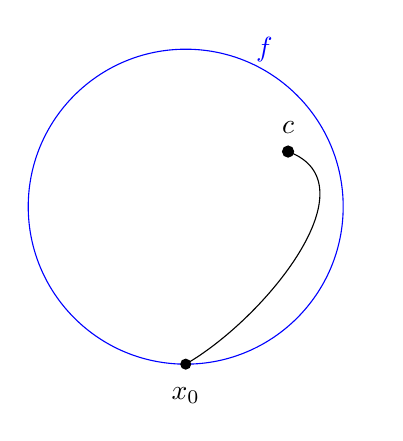
\begin{tikzpicture}
      \draw[blue] (0,0) circle (2);
      \fill (0, -2) circle (2pt);
      \draw (1.3, 0.7) circle (2pt);
      \draw (0,-2) to [out=30, in=-20] (1.3, 0.7);
      \fill (1.3, 0.7) circle (2pt);
      \node at (1.3, 1) {$c$};
      \node at (0,-2.4) {$x_0$};
      \node at (1, 2) {$\color{blue}f$};
    \end{tikzpicture}
  \end{center}

  Przestrzeń $X$ jest jednospójna, gdy jest drogowo spójna i ma trywialną grupę podstawową. Jednospójność w oczywisty sposób implikuje warunek $c)$ wyżej, z którego dostajemy, że dowolne dwa odwzorowania $S^1\to X$ są homotopijne z punktami stałymi, które możemy połączyć ($X$ łukowo spójne). 

  Z drugiej strony, jeśli dowolne dwa odwzorowania $S^1\to X$ są homotopijne, to w szczególności każde takie odwzorowanie jest homotopijne z odwzorowaniem stałym $x_0$ dla dowolnego $x_0\in X$. To daje łukową spójność $X$ oraz trywialność grupy podstawowej.
\end{solution}

\begin{problem}
  Jeśli $\pi_1X=0$, to każde dwie drogi łączące dowolnie wybrane dwa punkty $x_0, x_1\in X$ są homotopijne.
\end{problem}

\begin{solution}
  Niech $f, g$ będą drogami między $x_0$ a $x_1$. Wtedy $fg^{-1}$ będzie pętlą zbazowaną w $x_0$. Ponieważ $\pi_1X=0$, to $fg^{-1}\sim x_0$. Z zadania 2 wiemy, że wtedy $f\sim g$.
\end{solution}

\begin{problem}
  Mówimy, że przestrzeń topologiczna $X$ jest ściągalna, jeśli istnieje odwzorowanie $F:X\times I\to X$ takie, że $F(x, 0)=x$ oraz $F(x, 1)=x_0$ dla dowolnego $x$ oraz pewnego ustalonego $x_0$. Uzasadnij, że jeśli $X$ jest przestrzenią ściągalną, to jest też drogowo spójna, oraz $\pi_1X=0$ (innymi słowy, $X$ jest wtedy jednospójna).
\end{problem}

\begin{solution}
  Niech $x_1,x_2\in X$ będą dowolnymi punktami. Wówczas droga $f(t)=F(x_1, t)$ idzie z $x_1$ do $x_0$, a droga $g(t)=F(x_2, 1-t)$ idzie od $x_0$ do $x_2$. Łącząc obie te drogi dostajemy ścieżkę $x_1$ do $x_2$, czyli przestrzeń jest łukowo spójna.

  Weźmy teraz dowolną pętlę $f$ zbazowaną w punkcie $x_0$. Rozważmy homotopię $H(s, t)=F(f(s), t)$, która dla $t=0$ wynosi $f(s)$, a dla $t=1$ jest stale równa $x_0$. Z tego wynika, że $f\sim x_0$, czyli każda pętla jest homotopijna z elementem neutralnym $\pi_1X$ i grupa ta jest trywialna.
\end{solution}

\begin{problem}
  Uzasadnij, że każdy wypukły podzbiór w $\R^n$ jest ściągalny.
\end{problem}

\begin{solution}
  Wybierzmy dowolny punkt $x_0$ i z definicji zbioru wypukłego odcinek łączący $x_0$ z dowolnym innym punktem tego zbioru musi być zawarty w całości w tym zbiorze. Wystarczy napisać funkcję, która w sposób ciągły będzie przesuwać punkty po odcinkach łączących je z $x_0$.
\end{solution}

\begin{problem}
  Niech $T$ będzie skończonym \emph{drzewem}, tzn. spójnym skończonym grafem niezawierającym zamkniętych cykli krawędzi. Uzasadnij, że $\pi_1T=0$.
\end{problem}

\begin{solution}
  Jedyne pętle jakie znajdziemy w $T$ to pętla stała oraz pętle, które idą po wierzchołkach w jedną stronę i wracają po swoich śladach do punktu zaczepienia. Ten drugi rodzaj pętli to $ff^{-1}$ i jest homotopijne równy drodze stałej.
\end{solution}

\begin{problem}
  Uzasadnij, że homomorfizm $\phi_c:\pi_1(X, x_0)\to \pi_1(X, x_1)$ (związany ze zmianą punktu bazowego) zależy tylko od klasy homotopii drogi $d$ od $x_0$ do $x_1$.
\end{problem}


